\documentclass[12pt,a4paper,fleqn]{article} 
\usepackage[utf8]{inputenc} 
\usepackage{amsmath,amssymb,amsthm,mathtools} 
\usepackage{geometry} 
\usepackage{graphicx} 
\usepackage{microtype} 
\usepackage{enumitem} 
\usepackage{url} 
\usepackage{hyperref} 
\usepackage{booktabs} 
\usepackage{caption} 
\usepackage{subcaption} 
\usepackage{setspace} 
\usepackage{fancyvrb} 
\usepackage{tcolorbox} 

% --- Added for Times New Roman ---
\usepackage{newtxtext,newtxmath} 
% ---------------------------------

\tcbuselibrary{listings, breakable} 
\onehalfspacing 
\geometry{margin=1in} 
\hypersetup{colorlinks=true, citecolor=blue, linkcolor=black, urlcolor=blue}

% --- Font Settings: Times New Roman ---
\usepackage{newtxtext,newtxmath}

% Configure verbatim to break long lines
\fvset{breaklines=true, breakanywhere=true}

\title{Seasonal Trading Strategies: Identifying Optimal Entry and Exit Windows across NEPSE Sub-Sectors}
\author{Tek Raj Pant \and Himal Jung Oli \\
M.Sc. Computational Mathematics \quad M.Sc. Computational Statistics \\
School of Science, Department of Mathematics \\
Kathmandu University}
\date{June 2026}

\begin{document}

% -------- COVER PAGE --------
\begin{titlepage}
    \centering
    \vspace*{0cm}
    
\includegraphics[width=0.2\textwidth]{assets/ku-logo.jpg}\par\vspace{0.5cm}
    {\scshape\LARGE Kathmandu University \par}
    {\Large School of Science \par}
    {\large Department of Mathematics \par}
    \vspace{1cm}
    \rule{\linewidth}{0.8pt} \\[0.1cm]
    {\Huge \bfseries Seasonal Trading Strategies: Identifying Optimal Entry and Exit Windows across NEPSE Sub-Sectors \par}
    \vspace{0.3cm}
    \rule{\linewidth}{0.8pt} \\[1cm]
    {\Large \bfseries A Project Report \par}
    \vspace{0.2cm}
    {\Large \textbf{Authors:}\par}
    \vspace{0.2cm}
    {\large \textbf{Tek Raj Pant} \par}
    {\large \textbf{Himal Jung Oli} \par}
    {\large M.Sc. Computational Mathematics \par}
    {\large Computational Statistics \par}
    \vspace{0.8cm}
    {\Large \textbf{Submitted to:}\par}
    \vspace{0.2cm}
    {\large Professor Dr. Jyoti U. Devkota \par}
    \vspace{0.8cm}
    {\large \today}
\end{titlepage}

\newpage
\pagenumbering{arabic}
\setcounter{page}{1}

\section{Introduction}
The Nepal Stock Exchange (NEPSE) often exhibits patterns influenced by the Bikram Sambat calendar, fiscal year cycles, and major festivals like Dashain and Tihar \cite{shrestha2023seasonal}. This project explores the \textit{Seasonality Hypothesis} — that stock returns are not purely random but follow periodic trends that challenge weak-form efficiency \cite{joshi2025broad}. By analysing sectoral performance over five years, we distinguish genuine anomalies from noise \cite{basnet2022efficient}.

Different sub-sectors (banking, hydropower) show unique trends tied to fiscal year closings and festive windows \cite{gurung2024fiscal}. Our goal is to identify optimal entry and exit windows using historical data, building on prior work on calendar anomalies \cite{adhikari2024calendar, sharma2021investor}.

\section{Objectives}
\begin{enumerate}
    \item Identify statistically significant monthly/seasonal trends within NEPSE sub-sectors.
    \item Quantify risk-return profiles during high-volatility periods.
    \item Develop a Z-score based entry–exit framework.
\end{enumerate}

\section{Data Source}
Daily closing prices spanning from 2021 to 2026 were sourced from Nepse Alpha (\url{https://nepsealpha.com/nepse-data}). The dataset comprises the following six sectors:
\begin{itemize}
    \item Banking
    \item Hydropower
    \item Manufacturing
    \item Microfinance
    \item Non-Life Insurance
    \item Others
\end{itemize}

Daily asset returns are computed as follows:
\[
R_t = \frac{P_t^{\text{close}} - P_{t-1}^{\text{close}}}{P_{t-1}^{\text{close}}}
\]
where $P_t^{\text{close}}$ denotes the closing price at time $t$, and $P_{t-1}^{\text{close}}$ represents the closing price of the preceding trading day.
\section{Methodology}

This study employs a comprehensive suite of statistical and econometric techniques to investigate seasonal patterns in the daily returns of six NEPSE sub-sectors over the period 2021–2026. All analyses are conducted in the R statistical computing environment \cite{rcore2024} using a range of specialised packages (including \texttt{dplyr}, \texttt{ggplot2}, \texttt{lubridate}, \texttt{moments}, \texttt{boot}, \texttt{WRS2}, \texttt{lmPerm}, and \texttt{purrr}). The analytical framework progresses from exploratory data visualisation and distributional characterisation, through parametric and non-parametric hypothesis testing, to regression modelling and a battery of seasonality-detection procedures. For each method we state the substantive question it addresses, the underlying statistical model or test, the null hypothesis where applicable, and the manner in which the method is operationalised on our data.

\subsection{Exploratory Analysis}

Prior to formal inference, the structure and distribution of closing prices are examined graphically to identify potential outliers, assess the shape of the empirical distribution, and evaluate departures from normality that would influence the choice of subsequent tests.

\textbf{Boxplots} \cite{tukey1977eda} are constructed for closing prices stratified by sector using the \texttt{ggplot2} package with \texttt{geom\_boxplot()}. The box displays the interquartile range (IQR), with whiskers extending to the most extreme observation within \(1.5\times\text{IQR}\) from the quartiles; points beyond are flagged as potential outliers. This visualisation reveals the relative scale, spread, and skewness of prices across the six sectors and draws attention to extreme values that could distort parametric analyses.

\textbf{Histograms} with overlaid density curves, generated using \texttt{geom\_histogram()} from \texttt{ggplot2}, provide a first assessment of the shape of the closing-price distribution. Separate histograms are produced for each sector to examine symmetry, modality, and the presence of heavy tails. A bell-shaped reference aids the visual comparison with a normal density.

\textbf{Q–Q (quantile–quantile) plots} \cite{chambers1983graphical}, created using \texttt{stat\_qq()} and \texttt{stat\_qq\_line()}, compare sample quantiles against the theoretical quantiles of a standard normal distribution. Systematic departures from the diagonal line signal non-normality; in particular, an S-shaped or concave/convex pattern indicates heavy tails or skewness. These plots are instrumental in deciding between parametric and robust or non-parametric methods in subsequent stages.

\subsection{Distribution Analysis}

Daily simple returns are computed from closing prices as
\[
R_t = \frac{P_t^{\text{close}} - P_{t-1}^{\text{close}}}{P_{t-1}^{\text{close}}},
\]
and all distributional analyses are performed on this return series, after removing the first observation of each sector (which is undefined). Data manipulation for this calculation is performed using the \texttt{dplyr} package with \texttt{group\_by()}, \texttt{arrange()}, \texttt{mutate()}, and \texttt{lag()} functions. Classical financial models often assume that asset returns are normally distributed; however, empirical returns frequently exhibit skewness and excess kurtosis \cite{cont2001empirical}. We therefore quantify these higher moments and apply a formal normality test.

\textbf{Skewness} measures the degree of asymmetry of the return distribution. The sample skewness is
\begin{equation}
g_1 = \frac{1}{n}\sum_{i=1}^{n}\Big(\frac{x_i - \bar{x}}{s}\Big)^3,
\label{eq:skewness}
\end{equation}
where \(s\) denotes the sample standard deviation \cite{joanes1998comparing}. A positive (negative) skewness indicates a longer right (left) tail, i.e. a higher probability of large positive (negative) returns relative to a symmetric distribution. The skewness and kurtosis statistics are computed using the \texttt{skewness()} and \texttt{kurtosis()} functions from the \texttt{moments} package.

\textbf{Kurtosis} quantifies the heaviness of the tails compared with a normal distribution. We employ the excess kurtosis,
\begin{equation}
g_2 = \frac{1}{n}\sum_{i=1}^{n}\Big(\frac{x_i - \bar{x}}{s}\Big)^4 - 3,
\label{eq:kurtosis}
\end{equation}
so that a normal distribution has zero excess kurtosis \cite{de1992tests}. Positive values (leptokurtic) imply fatter tails and a greater propensity for extreme events than the normal model would predict.

\textbf{Shapiro–Wilk Test} \cite{shapiro1965variance} is used to formally test whether the sector-wise return data follow a normal distribution. The test is applied using the \texttt{shapiro.test()} function from the base R \texttt{stats} package. The test statistic \(W\) is
\begin{equation}
W = \frac{\big(\sum_{i=1}^{n} a_i x_{(i)}\big)^2}{\sum_{i=1}^{n} (x_i - \bar{x})^2},
\label{eq:shapiro}
\end{equation}
where \(x_{(i)}\) are the order statistics and the coefficients \(a_i\) depend on the expected values of normal order statistics. The null hypothesis is
\[
H_0: \text{The data are drawn from a normal distribution.}
\]
A rejection of \(H_0\) at the 5\% significance level indicates significant deviation from normality. In our analysis the test is applied to the daily returns of each sector separately. The strong rejection for all sectors (\(p<10^{-12}\)) provides the primary justification for the use of robust and non-parametric methods alongside conventional parametric tests.

\subsection{Confirmatory Analysis}

Having established that returns are non-normal, we proceed to test for associations between returns, calendar months, and sectors using a blend of parametric and non-parametric approaches.

\subsubsection{Chi-square Test of Independence}

We examine whether the direction of a daily return (gain or loss) is related to the calendar month in which it occurs. Each daily return is categorised as ``Gain'' if \(R_t>0\) and ``Loss'' otherwise. The month of the observation is extracted from the date using the \texttt{month()} function from the \texttt{lubridate} package. A \(2\times12\) contingency table of observed frequencies is constructed using \texttt{table()}, and the chi-square test of independence \cite{pearson1900chi} is applied via \texttt{chisq.test()}. The null hypothesis is
\[
H_0: \text{Return direction and month are independent.}
\]
The test statistic is
\begin{equation}
\chi^2 = \sum_{i,j} \frac{(O_{ij} - E_{ij})^2}{E_{ij}},
\label{eq:chisq}
\end{equation}
where \(O_{ij}\) are the observed counts and \(E_{ij}\) the expected counts under independence. Under \(H_0\), \(\chi^2\) asymptotically follows a chi-squared distribution with \((r-1)(c-1)\) degrees of freedom. A significant result would indicate that the likelihood of a positive or negative day varies systematically by month, providing preliminary evidence of seasonality.

\subsubsection{One-Way Analysis of Variance (ANOVA)}

To evaluate whether the average daily return differs across months (or across sectors), we employ one-way ANOVA \cite{fisher1925statistical} using the \texttt{aov()} function from base R. The model posits
\[
y_{ij} = \mu + \alpha_j + \varepsilon_{ij},
\]
where \(\mu\) is the overall mean, \(\alpha_j\) is the fixed effect of the \(j\)-th group (e.g., month), and \(\varepsilon_{ij}\sim N(0,\sigma^2)\). The null hypothesis is that all group effects are zero,
\[
H_0: \alpha_1 = \alpha_2 = \dots = \alpha_k = 0,
\]
against the alternative that at least one group mean differs. The \(F\)-statistic,
\begin{equation}
F = \frac{\text{MS}_{\text{between}}}{\text{MS}_{\text{within}}},
\label{eq:F}
\end{equation}
compares the variation between group means to the variation within groups. In our study, the grouping variable for the ``by month'' ANOVA is the month of the year (created from the date using \texttt{month()} from \texttt{lubridate}), and for the ``by sector'' ANOVA it is the sector identifier. Because the normality assumption is clearly violated, these parametric ANOVA results are interpreted with caution and are supplemented by the robust and non-parametric procedures described below.

\subsubsection{Two-Way ANOVA (Sector \(\times\) Month)}

To assess whether any monthly seasonality differs across sectors, we fit a two-way ANOVA model with interaction \cite{kutner2005applied}:
\[
y_{ijk} = \mu + \alpha_i + \beta_j + (\alpha\beta)_{ij} + \varepsilon_{ijk},
\]
where \(\alpha_i\) is the sector effect, \(\beta_j\) the month effect, and \((\alpha\beta)_{ij}\) the interaction between sector and month. The model is estimated using \texttt{aov()} with the formula \texttt{Return \textasciitilde{} Symbol * MonthFactor}. A significant interaction term would indicate that the monthly pattern of returns is not uniform across sectors, warranting sector-specific trading strategies. The significance of each term is tested via the corresponding \(F\)-ratio.

\subsection{Non-Parametric Tests}

Given the strong rejection of normality for all sectors, we complement the parametric ANOVA with rank-based tests that do not assume a specific distribution.

\subsubsection{Kruskal–Wallis Rank Sum Test}

The Kruskal–Wallis test \cite{kruskal1952use}, implemented via \texttt{kruskal.test()} from base R, is the non-parametric analogue of one-way ANOVA. It tests the null hypothesis that all groups have the same median. The test statistic is
\begin{equation}
H = \frac{12}{N(N+1)} \sum_{j=1}^{k} \frac{R_j^2}{n_j} - 3(N+1),
\label{eq:kruskal}
\end{equation}
where \(R_j\) is the sum of ranks in group \(j\), \(n_j\) is the group size, and \(N\) is the total number of observations. Under \(H_0\), \(H\) approximately follows a \(\chi^2_{k-1}\) distribution. We apply the test separately to compare return medians across sectors and across months. A significant result indicates that at least one group median differs, confirming the presence of a month or sector effect without relying on normality.

\subsubsection{Mann–Whitney \(U\) Test}

For pairwise comparisons between two independent groups (e.g., Banking versus Others), we use the Mann–Whitney \(U\) test \cite{mann1947test}, implemented via \texttt{wilcox.test()} from base R. The test compares the distributions of the two groups based on the ranks of the combined sample. The null hypothesis is that the two groups have identical distributions. The two-sided \(p\)-value is obtained from the large-sample normal approximation. This test allows us to assess, for example, whether the return distribution of the Banking sector differs significantly from that of the Others sector.

\subsection{Mathematical Modelling}

\subsubsection{Simple Linear Regression}

To detect a possible linear time trend in daily returns, we fit the model using \texttt{lm()} from base R:
\[
R_t = \beta_0 + \beta_1 \cdot t + \varepsilon_t,\quad \varepsilon_t \sim N(0,\sigma^2),
\]
where \(t\) is a numerical index representing the number of days since the start of the sample period (converted using \texttt{as.numeric(Date)}). The parameters \(\beta_0\) and \(\beta_1\) are estimated by ordinary least squares, and the statistical significance of the slope coefficient \(\beta_1\) is tested using a \(t\)-test \cite{draper1998applied}. A significant positive (negative) slope would indicate a systematic upward (downward) drift over time, which must be distinguished from seasonal patterns.

\subsubsection{Multiple Linear Regression (Autoregressive)}

To assess whether lagged returns or sector membership carry predictive power, we estimate an autoregressive model with a categorical sector variable using \texttt{lm()}:
\[
R_t = \beta_0 + \beta_1 R_{t-1} + \beta_2 \text{Sector} + \varepsilon_t.
\]
The lagged return \(R_{t-1}\) is created using \texttt{lag()} from \texttt{dplyr}, allowing us to test for first-order autocorrelation, a common feature of financial time series that could confound seasonal signals. The sector dummy variables capture systematic differences in average returns across sectors. The model is estimated via ordinary least squares, and residual diagnostics are examined for heteroscedasticity and autocorrelation to assess model adequacy.

\subsection{Seasonality Detection}

A multi-faceted set of techniques is deployed to pinpoint and validate seasonal patterns in the return data.

\subsubsection{Monthly Ranking Metrics}

For each sector and month, we compute four descriptive measures using \texttt{dplyr}'s \texttt{group\_by()} and \texttt{summarise()} that provide a comprehensive view of performance:
\begin{itemize}
    \item \textbf{Mean return} \(\bar{R}_{s,m}\) — the arithmetic average of daily returns in month \(m\) for sector \(s\).
    \item \textbf{Median return} — a robust measure of central tendency less affected by outliers.
    \item \textbf{Win ratio} — the proportion of trading days within the month that yield a positive return: \(\frac{1}{n_{s,m}}\sum \mathbb{I}(R>0)\).
    \item \textbf{Sharpe ratio} \cite{sharpe1966mutual} — the mean return divided by its standard deviation, \(\text{SR}_{s,m} = \frac{\bar{R}_{s,m}}{\sigma_{s,m}}\), measuring risk-adjusted performance.
\end{itemize}
Months are then ranked within each sector by their mean return using \texttt{slice\_max()} and \texttt{slice\_min()} from \texttt{dplyr}. The top two and bottom two months are extracted to identify the most favourable entry and exit periods.

\subsubsection{Z-Score Entry/Exit Framework}

To generate actionable trading signals, we standardise daily returns within each sector–month combination using \texttt{mutate()} and \texttt{group\_by()} from \texttt{dplyr}. For sector \(s\) and month \(m\), let \(\mu_{s,m}\) and \(\sigma_{s,m}\) denote the historical mean and standard deviation of daily returns. The Z-score on day \(t\) is
\[
Z_{s,m,t} = \frac{R_{s,m,t} - \mu_{s,m}}{\sigma_{s,m}}.
\]
We flag any observation with \(|Z| > 1.5\) as an extreme event. A strongly negative Z-score (\(Z < -1.5\)) suggests that the return is unusually low relative to its historical distribution for that sector–month, potentially indicating an oversold condition and a buying opportunity (ENTRY signal). Conversely, a strongly positive Z-score (\(Z > +1.5\)) suggests an overbought condition and a candidate for exit (EXIT signal) \cite{tsay2010analysis}. Because the return distributions exhibited substantial kurtosis, we also consider a more conservative threshold of \(\pm 1.8\) to reduce the likelihood of false signals driven by fat tails. The frequency and average magnitude of signals are compiled by month and sector using \texttt{summarise()}.

\subsubsection{Cumulative Return by Day-of-Year}

To determine the historically optimal day to close a position, we first compute the average daily return for each calendar day (day 1 through 365) across all years and sectors using \texttt{yday()} from \texttt{lubridate}, followed by \texttt{group\_by()} and \texttt{summarise()}. The cumulative average return up to day \(d\) is
\[
C(d) = \sum_{k=1}^{d} \bar{R}_k,
\]
where \(\bar{R}_k\) is the mean return on the \(k\)-th day of the year, calculated using \texttt{cumsum()}. The day \(d^*\) that maximises \(C(d)\) is the point at which a strategy that entered at the start of the year would have achieved its highest cumulative profit on average. We report \(d^*\) and its approximate calendar date for each sector as the optimal exit day, extracted using \texttt{slice\_max()}.

\subsubsection{Year-on-Year Consistency}

A seasonal pattern is only practically useful if it recurs reliably across different years. We assess reliability by calculating, for each sector and month, the proportion of years in which the total monthly return was positive:
\[
\text{Consistency}_{s,m} = \frac{\#\{\text{years with positive total return in month } m\}}{\text{total years}}.
\]
A consistency rate of \(0.8\) or higher is adopted as the threshold for a dependable seasonal window \cite{lakonishok1988seasonal}. Only months with at least three years of data are considered to ensure robustness. This analysis is performed using \texttt{year()} and \texttt{month()} from \texttt{lubridate}, with \texttt{group\_by()} and \texttt{summarise()} from \texttt{dplyr}.

\subsubsection{Bootstrap Confidence Intervals}

Classical \(t\)-based confidence intervals for the mean assume normality and can be misleading for heavy-tailed return data. We therefore construct 95\% percentile bootstrap confidence intervals for the mean return of each sector–month combination using the non-parametric bootstrap \cite{efron1994introduction} via the \texttt{boot()} function from the \texttt{boot} package, with a user-defined \texttt{boot\_mean()} function. For a given sector–month, we draw 1000 resamples with replacement from the observed daily returns, compute the mean of each resample, and take the 2.5th and 97.5th percentiles of the resulting bootstrap distribution as the lower and upper confidence limits using \texttt{boot.ci()} with \texttt{type = "perc"}. An interval that does not contain zero provides evidence of a non-zero mean return for that month.

\subsubsection{Robust ANOVA (Trimmed Means)}

To further mitigate the influence of outliers and the pronounced tails, we perform a one-way ANOVA on 20\% trimmed means using the \texttt{t1way()} function from the \texttt{WRS2} package \cite{wilcox2017introduction}. Trimming removes the most extreme observations from each tail before computing the group means, yielding a test that is resistant to violations of normality and heterogeneity of variance. The test statistic \(F_t\) (a Welch–James-type statistic) is used to evaluate the null hypothesis that all population trimmed means are equal across months. Effect size \(\hat{\eta}\) is estimated and accompanied by a bootstrap confidence interval.

\subsubsection{Permutation Test}

As a fully distribution-free validation of the month effect, we conduct a permutation test \cite{good2005permutation} using the \texttt{aovp()} function from the \texttt{lmPerm} package. The \(F\)-statistic from a one-way ANOVA (by month) is computed on the original data. The month labels are then randomly shuffled 5000 times, and the same \(F\)-statistic is recalculated for each permuted dataset. The permutation \(p\)-value is the proportion of permuted \(F\)-values that exceed the observed \(F\). Because this test makes no distributional assumptions, it provides a robust check on the statistical significance of the monthly seasonality.

All seasonality detection methods are applied sector by sector, and their results are integrated to form a coherent picture of calendar-based return patterns. The combination of graphical, parametric, non-parametric, robust, and resampling techniques ensures that the conclusions are not the product of a single modelling choice but are supported by converging lines of evidence.

\vspace{15cm}
\section{Results and Discussion}

This section presents the empirical findings obtained from applying the statistical and econometric methods described in the Methodology section. The results are organised sequentially, beginning with exploratory diagnostics and progressing through confirmatory tests, seasonality detection techniques, and robustness checks. Each result is interpreted in light of the underlying hypotheses and the methodological choices that guided the analysis.

\subsection{Exploratory Data Analysis and Normality Assessment}

Figure~\ref{fig:boxplot} displays side-by-side boxplots of closing prices for the six NEPSE sub-sectors. The wide range of prices and the presence of numerous outliers (points beyond the whiskers) are immediately apparent. Sectors such as Hydropower and Others exhibit larger interquartile ranges, indicating greater cross-sectional dispersion in price levels. The boxplots also reveal mild positive skewness in several sectors, consistent with the well-known empirical regularity that equity price distributions are often right-skewed.

\begin{figure}[ht]
\centering
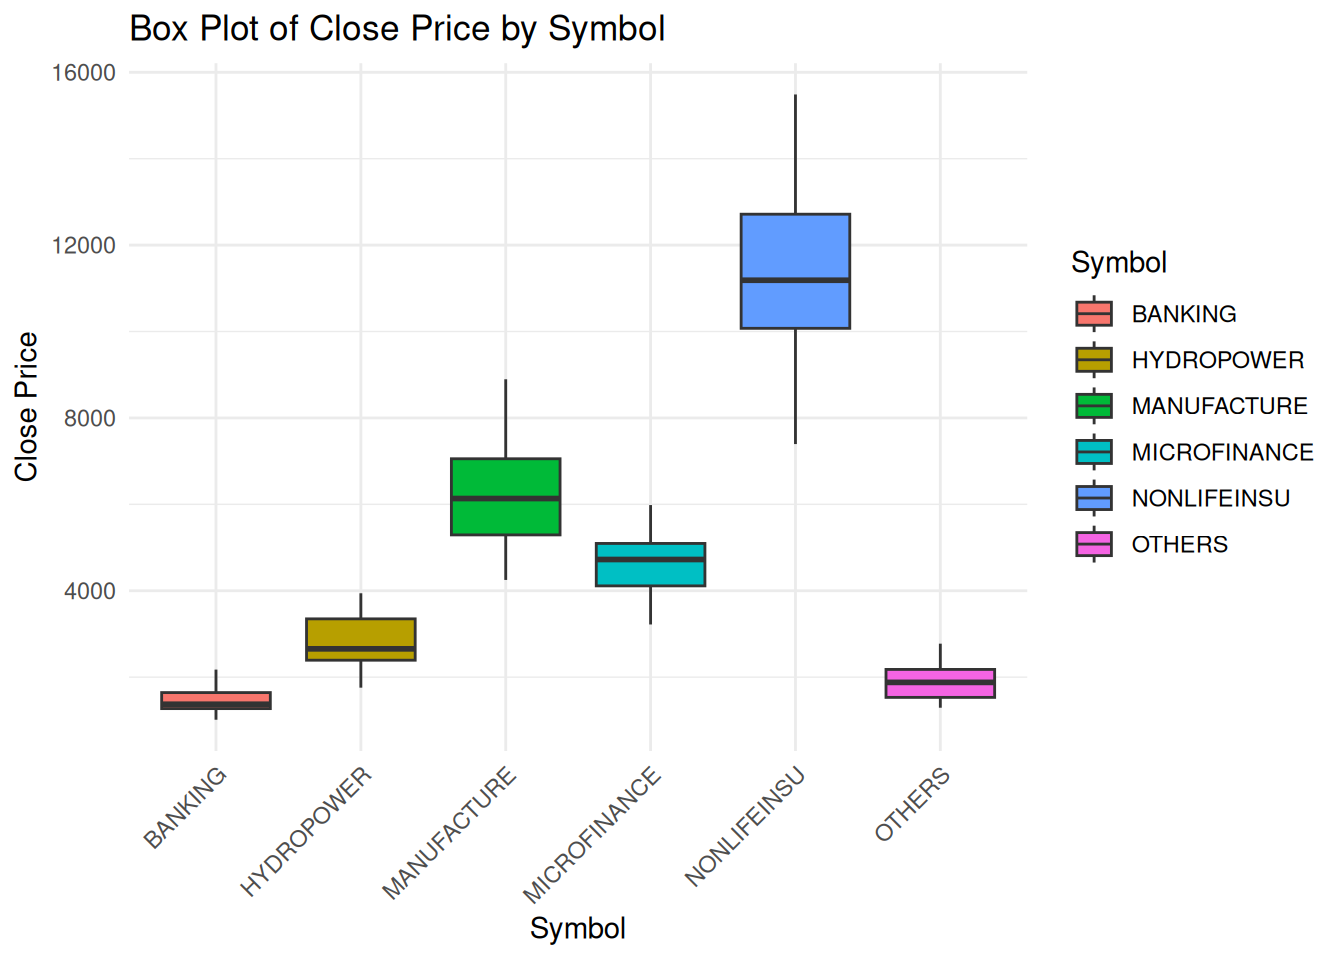
\includegraphics[width=0.95\textwidth]{figures/stats-box-plot.png}
\caption{Box plots of closing prices by sector. Outliers are marked as individual points beyond \(1.5\times\text{IQR}\) from the quartiles.}
\label{fig:boxplot}
\end{figure}

Figure~\ref{fig:qq} presents the normal Q–Q plots for each sector. Systematic curvature away from the reference line, especially in the upper and lower tails, provides strong graphical evidence against the assumption of normally distributed closing prices. All sectors exhibit heavy-tailed behaviour, with both the lower and upper extremes deviating markedly from the theoretical normal quantiles. This visual diagnosis motivated the formal distributional tests that follow.

\begin{figure}[ht]
\centering
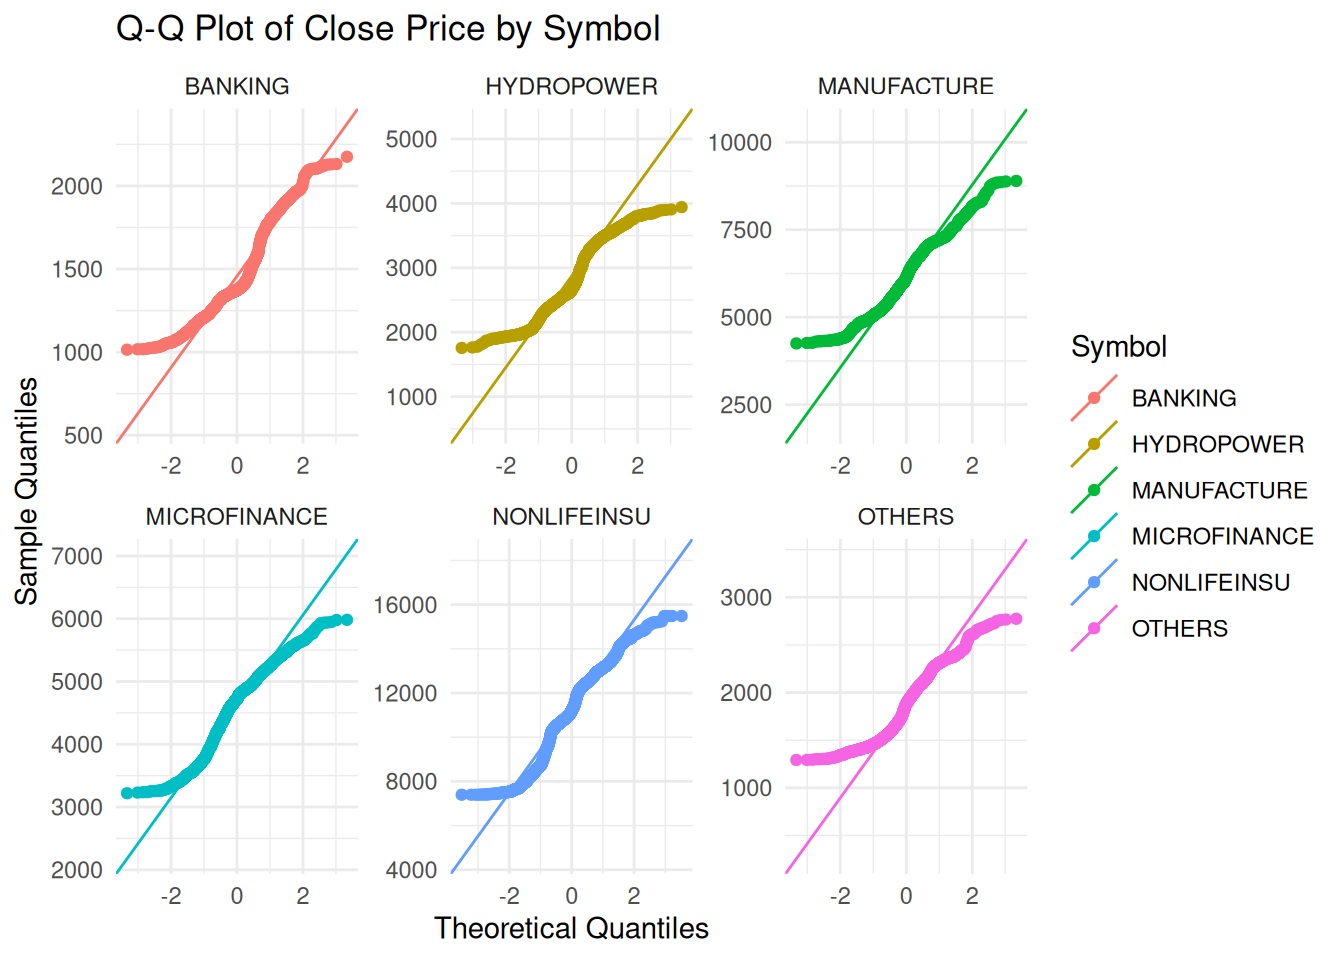
\includegraphics[width=0.95\textwidth]{figures/stats-q-q-plot.png}
\caption{Q–Q plots of closing prices by sector. Deviations from the diagonal indicate departures from normality, particularly in the tails.}
\label{fig:qq}
\end{figure}

Table~\ref{tab:distribution} reports the first four moments of the daily return distributions for each sector, calculated using the formulae for skewness and excess kurtosis. All sectors show positive skewness, ranging from 0.615 (Hydropower) to 1.14 (Banking), implying a tendency towards occasional large positive returns. Excess kurtosis values are substantially above zero in every sector, with Banking (8.24) and Non-Life Insurance (9.88) exhibiting the heaviest tails. These findings align with the stylised facts of financial returns documented by \cite{cont2001empirical} and indicate a far higher probability of extreme daily movements than a normal distribution would imply.

\begin{table}[ht]
\centering
\caption{Distributional characteristics of daily returns by sector}
\label{tab:distribution}
\begin{tabular}{lrrrr}
\toprule
Sector & Mean & SD & Skewness & Excess Kurtosis \\
\midrule
BANKING       & $-0.000117$ & 0.0132 & 1.140 & 8.24 \\
HYDROPOWER    & $\hphantom{-}0.000770$ & 0.0209 & 0.615 & 4.44 \\
MANUFACTURE   & $\hphantom{-}0.000458$ & 0.0162 & 0.798 & 4.83 \\
MICROFINANCE  & $\hphantom{-}0.000365$ & 0.0164 & 0.802 & 6.58 \\
NONLIFEINSU   & $\hphantom{-}0.000723$ & 0.0114 & 0.976 & 9.88 \\
OTHERS        & $\hphantom{-}0.000376$ & 0.0184 & 0.638 & 4.87 \\
\bottomrule
\end{tabular}
\end{table}

The Shapiro–Wilk test \cite{shapiro1965variance} was applied sector-wise to the daily returns. For every sector, the null hypothesis of normality was rejected with \(p < 10^{-12}\). This overwhelming evidence of non-normality justifies the adoption of non-parametric and robust methods in subsequent analyses. It also cautions against interpreting conventional ANOVA \(F\)-tests in isolation, despite their use as initial screening tools.

\subsection{Additional Exploratory Visualizations}

To gain deeper insights into the return distributions and temporal dynamics, we constructed several additional plots.

\subsubsection{Monthly Average Returns with Confidence Intervals}

Figure~\ref{fig:monthly_bar} displays a bar plot of mean daily returns for each sector by month, with 95\% bootstrap confidence intervals. The red horizontal line at zero serves as a visual reference for statistical significance. The plot clearly shows that July stands out with the highest mean returns across all sectors, while August and September consistently exhibit negative means. The confidence intervals for July are mostly above zero, confirming the robustness of this seasonal peak.

\begin{figure}[ht]
\centering
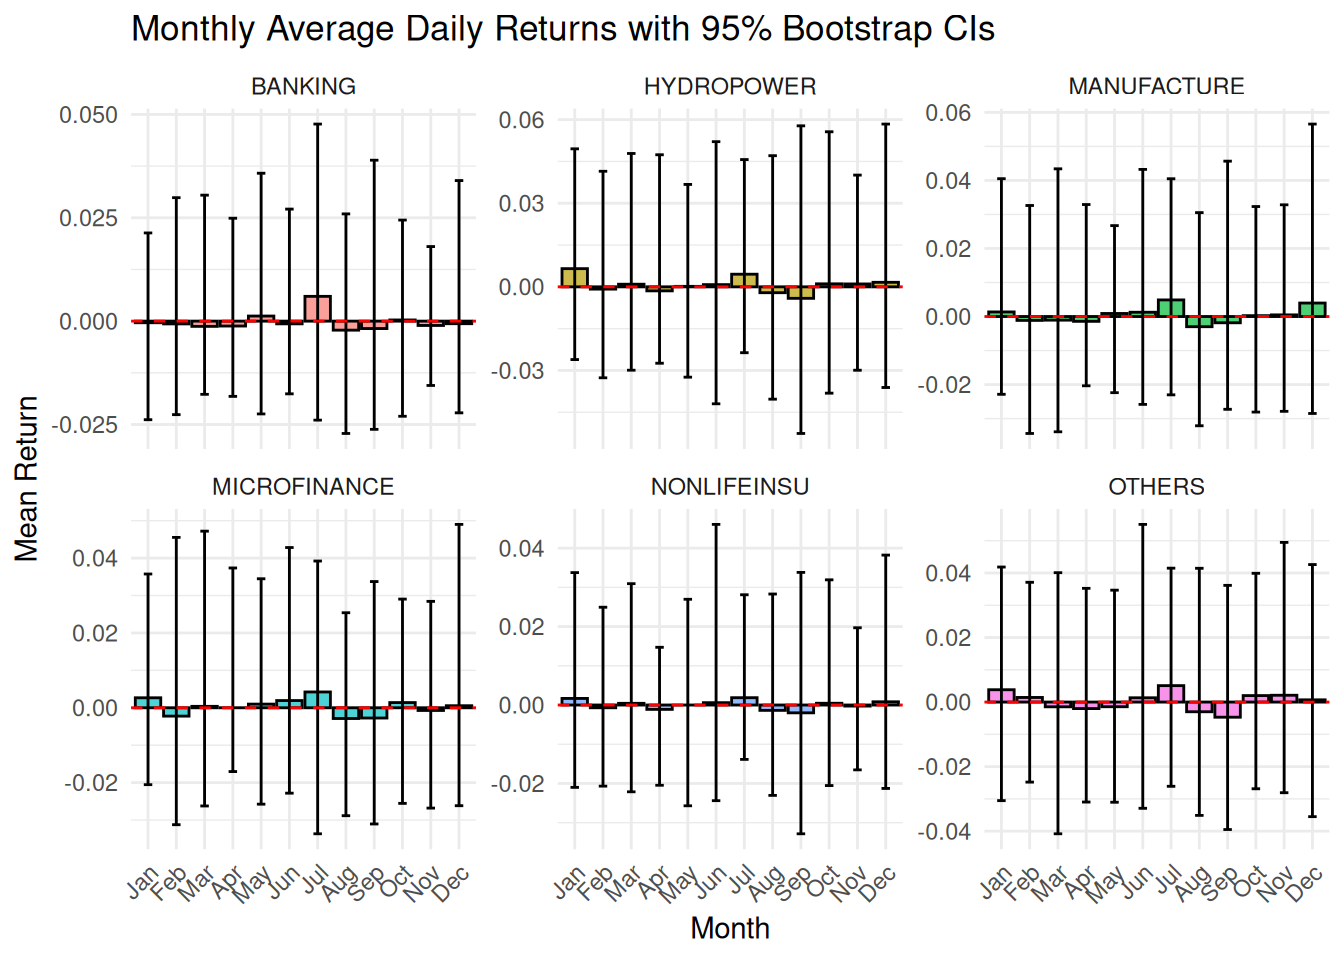
\includegraphics[width=0.95\textwidth]{figures/stats-monthly-bar.png}
\caption{Monthly average daily returns with 95\% bootstrap confidence intervals. Bars above the red line indicate statistically positive months.}
\label{fig:monthly_bar}
\end{figure}

\subsubsection{Density Plots of Returns with Normal Reference}

Figure~\ref{fig:density} shows kernel density estimates of daily returns for each sector, overlaid with a dotted red normal curve. The heavy tails and peakedness are visually evident; the empirical distributions are far more concentrated around zero with fatter tails than the normal reference. This reinforces the need for robust statistical methods that are not sensitive to extreme observations.

\begin{figure}[ht]
\centering
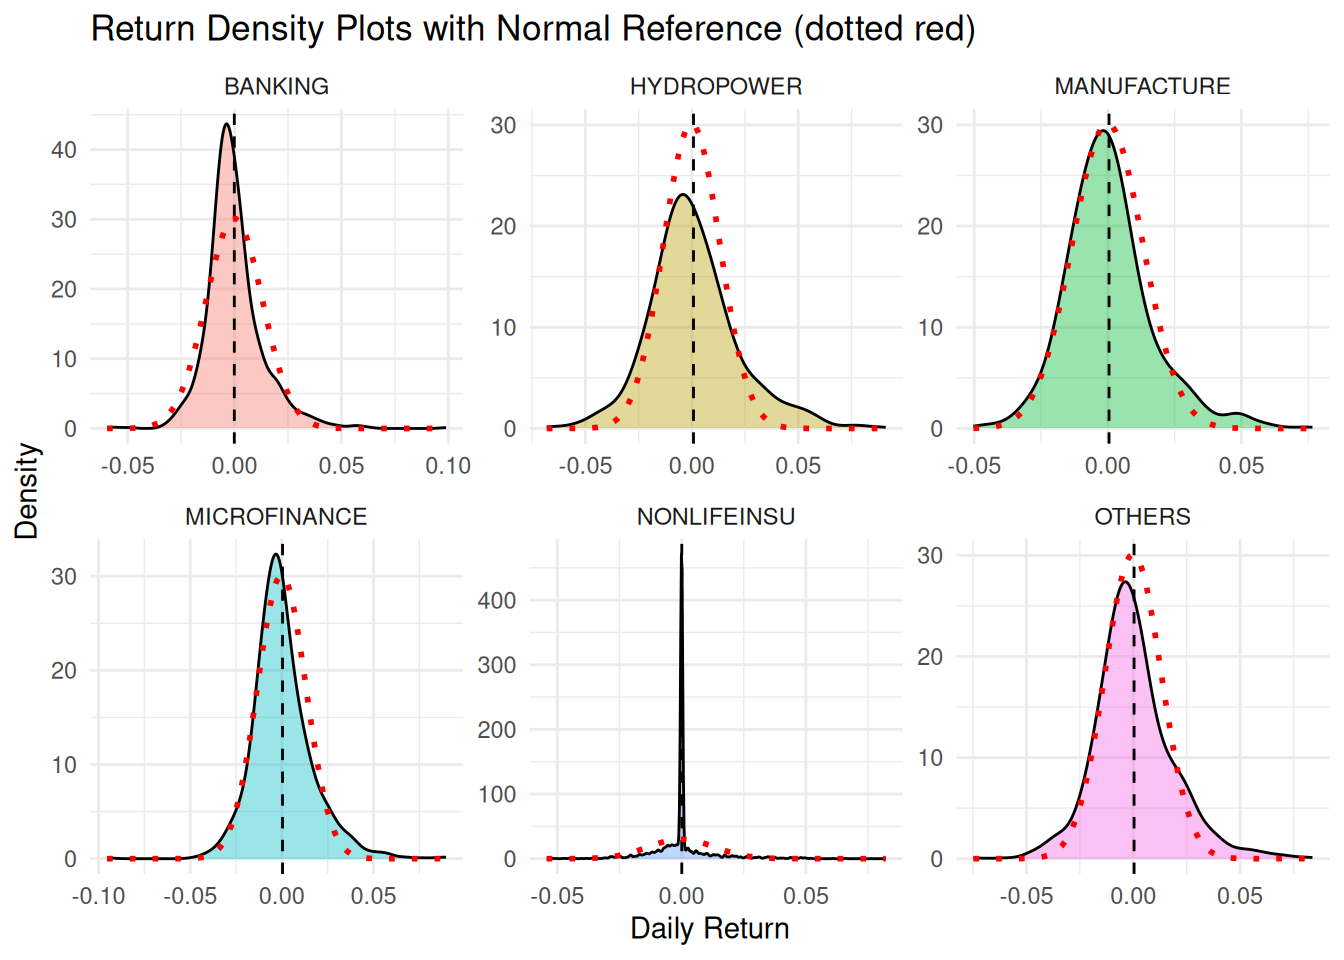
\includegraphics[width=0.95\textwidth]{figures/stats-density.png}
\caption{Density plots of daily returns by sector with a normal distribution reference (dotted red).}
\label{fig:density}
\end{figure}

\subsubsection{Time Series of Cumulative Returns}

Figure~\ref{fig:cumulative_ts} plots the cumulative sum of daily returns over the entire sample period (2021–2026) for each sector. The upward or downward trends reveal overall performance. Hydropower shows the strongest cumulative gain, while Banking exhibits a more modest upward drift. The plot also helps identify periods of sustained growth or decline, which may be linked to seasonal events.

\begin{figure}[ht]
\centering
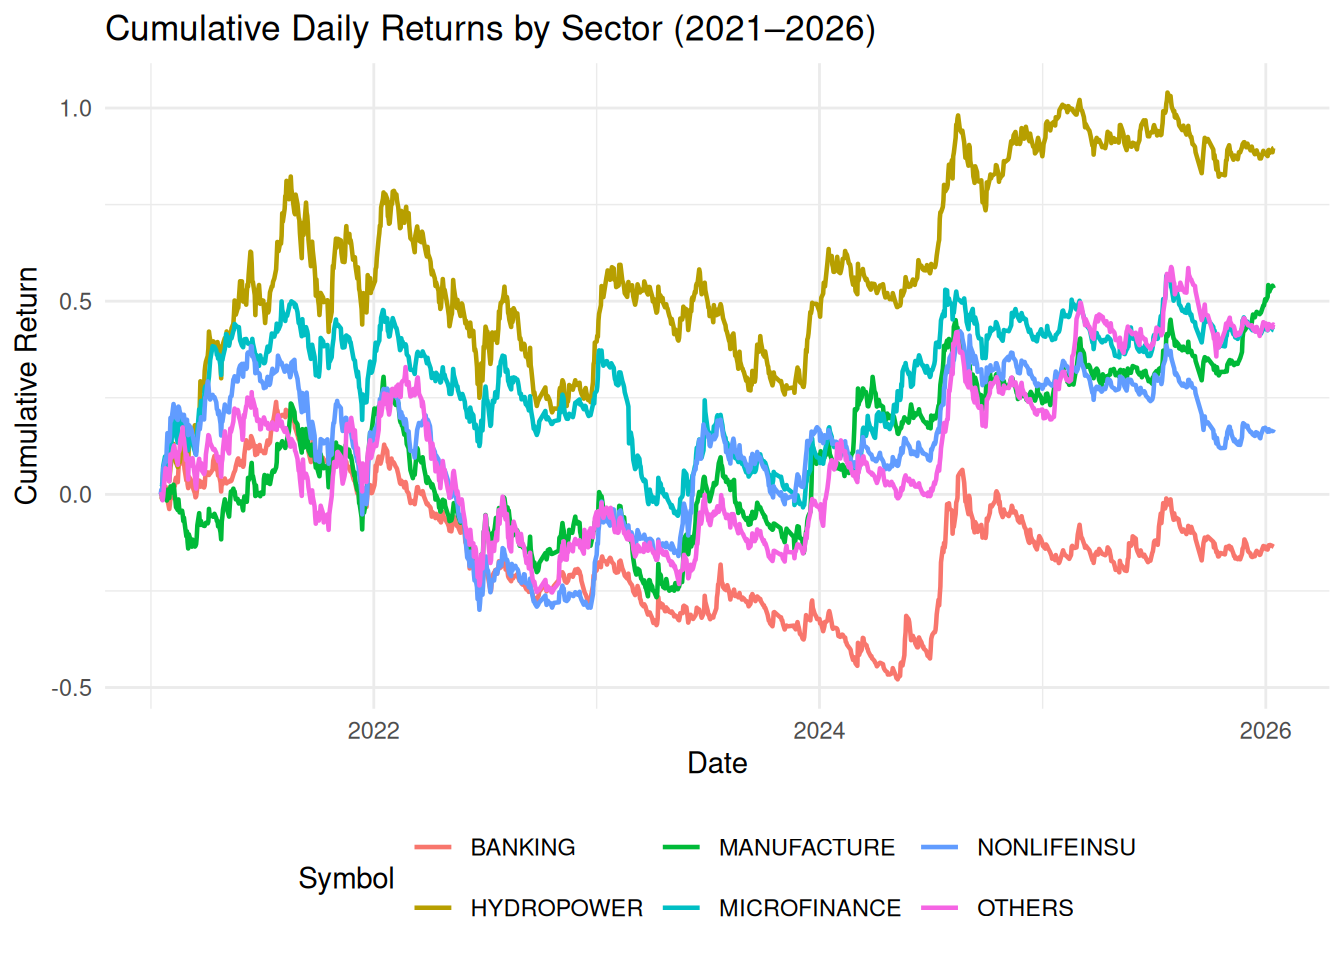
\includegraphics[width=0.95\textwidth]{figures/stats-cumulative-ts.png}
\caption{Cumulative daily returns over time by sector (2021–2026).}
\label{fig:cumulative_ts}
\end{figure}

\subsubsection{Heatmap of Mean Returns by Sector and Month}

Figure~\ref{fig:heatmap} presents a colour-coded matrix of mean returns for each sector–month combination. Red indicates negative returns, blue positive, and white near zero. The heatmap immediately highlights July as the warmest month across all sectors (deep blue), while August and September are predominantly red. This visualisation confirms the uniformity of the seasonal pattern across sectors, supporting the two‑way ANOVA result of a non‑significant interaction.

\begin{figure}[ht]
\centering
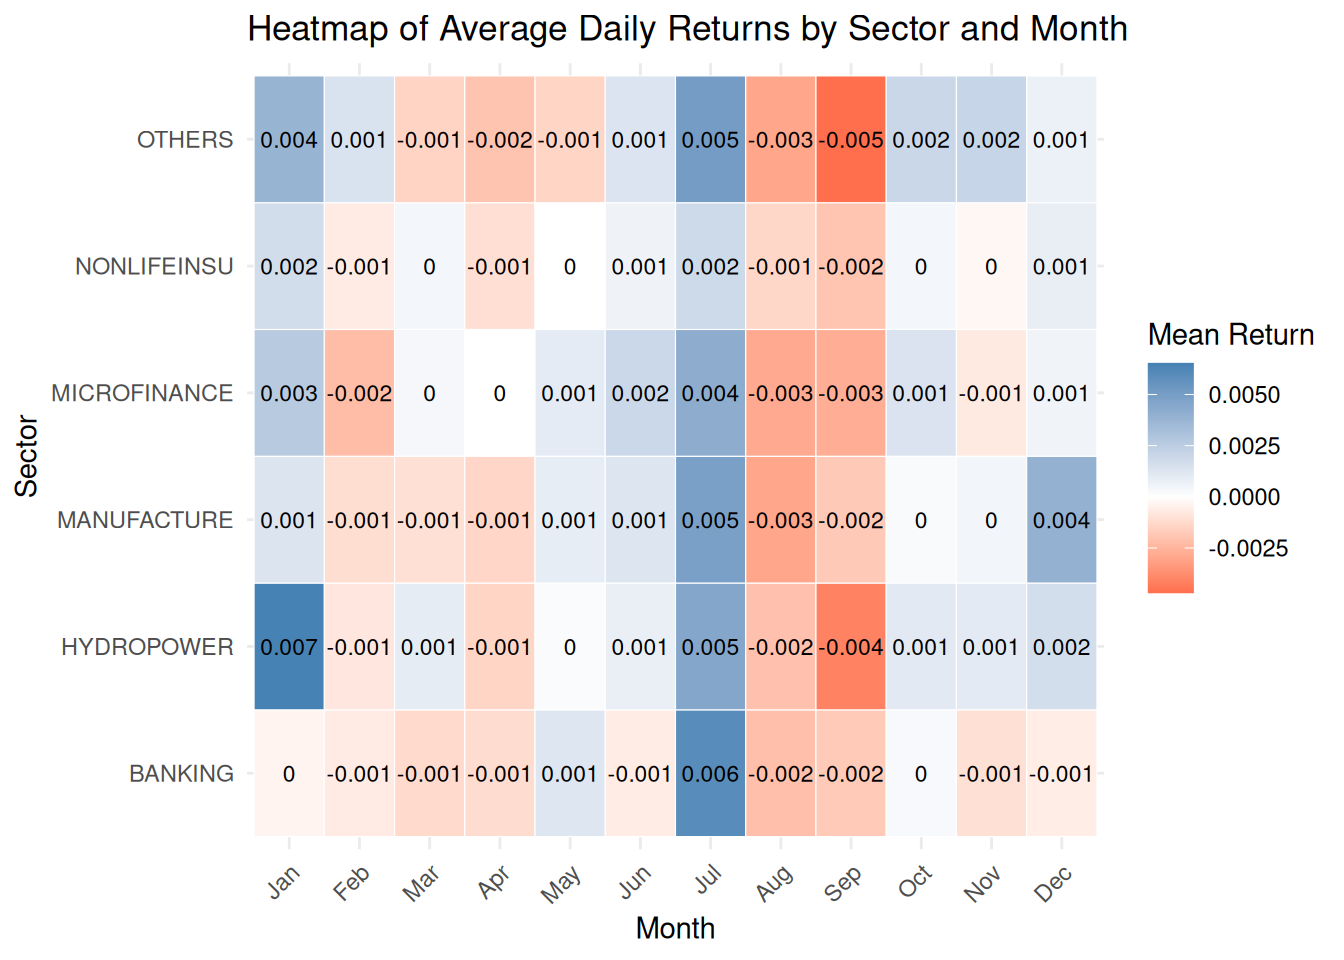
\includegraphics[width=0.95\textwidth]{figures/stats-heatmap.png}
\caption{Heatmap of average daily returns by sector and month. Blue = positive, red = negative.}
\label{fig:heatmap}
\end{figure}


\subsection{Month and Sector Effects}

A series of hypothesis tests was performed to determine whether return behaviour is associated with calendar months or sector membership.

\subsubsection{Chi-square Test of Independence}

The contingency table of return direction (Gain/Loss) versus month yielded a chi-square statistic of \(\chi^2(11) = 92.578\) with \(p = 5.2\times10^{-15}\). This result strongly rejects the null hypothesis that the direction of daily returns is independent of the calendar month. It indicates that the proportion of positive days varies systematically across the year, providing initial parametric evidence of seasonality.

\subsubsection{One-Way Analysis of Variance (ANOVA)}

The \(F\)-test comparing mean returns across the twelve months gave \(F(11,\, \text{large }df) = 10.46\), \(p < 2\times10^{-16}\), implying significant differences among monthly mean returns. Although the normality assumption is violated, the large sample size provides some robustness to the \(F\)-test; nonetheless, the result is corroborated by non-parametric and robust methods below.

A similar test of mean returns across the six sectors produced \(F(5,\, \text{large }df) = 0.497\) with \(p = 0.779\), indicating no significant differences in average daily returns among sectors. This suggests that any seasonal patterns are not confounded by systematic sectoral outperformance over the full sample period.

\subsubsection{Kruskal–Wallis Rank Sum Test}

The non-parametric analogue to one-way ANOVA yielded \(H(5) = 14.798\), \(p = 0.01126\). While significant at the 5\% level, this result is markedly weaker than the month effect, indicating that rank differences among sectors exist but are subtle. The Kruskal–Wallis test therefore captures a weak sector effect that the parametric ANOVA missed, likely because of distributional peculiarities.

\subsubsection{Mann–Whitney \(U\) Test}

A direct pairwise comparison of return distributions between the Banking and Others sectors resulted in a \(p\)-value of 0.8648, failing to reject the null of equal distributions. This reinforces the conclusion that, once calendar effects are accounted for, sectoral differences in daily returns are negligible.

Overall, these tests converge on a clear message: there is strong statistical evidence for monthly seasonality, but little evidence of persistent differences across sectors. Consequently, the search for optimal entry and exit windows can reasonably focus on a common calendar while allowing for minor sector-specific adjustments.

\subsection{Best and Worst Months}

Table~\ref{tab:bestmonths} reports the two best-performing months for each sector, ranked by mean daily return. The metrics include the mean, median, win ratio, and Sharpe ratio. The month of July (Shrawan) appears as the top month for five of the six sectors; the only exception is Hydropower, where January attains the highest mean return. Even in Hydropower, July ranks second. July exhibits consistently high win ratios (above 0.60 for Banking, Manufacturing, and Others) and positive Sharpe ratios, indicating that the superior mean return is not merely driven by a few outliers.

January emerges as the second-best month for Hydropower, Microfinance, Non-Life Insurance, and Others, suggesting a secondary seasonal window at the start of the calendar year. The median returns in these months are also positive or near zero, confirming that the favourable performance is broad-based rather than skewed by extreme values.

\begin{table}[ht]
\centering
\caption{Two best months per sector (ranked by mean daily return)}
\label{tab:bestmonths}
\begin{tabular}{lcccc}
\toprule
Sector & Month & Mean Return & Median Return & Win Ratio & Sharpe Ratio \\
\midrule
BANKING       & July    & 0.00599 & 0.00196 & 0.602 & 0.323 \\
BANKING       & May     & 0.00123 & -0.00087 & 0.464 & 0.096 \\
\addlinespace
HYDROPOWER    & January & 0.00653 & 0.00344 & 0.594 & 0.339 \\
HYDROPOWER    & July    & 0.00453 & 0.00444 & 0.540 & 0.241 \\
\addlinespace
MANUFACTURE   & July    & 0.00488 & 0.00407 & 0.628 & 0.305 \\
MANUFACTURE   & December & 0.00396 & 0.00212 & 0.557 & 0.197 \\
\addlinespace
MICROFINANCE  & July    & 0.00423 & 0.00322 & 0.566 & 0.242 \\
MICROFINANCE  & January & 0.00267 & -0.00044 & 0.475 & 0.178 \\
\addlinespace
NONLIFEINSU   & July    & 0.00187 & 0.00000 & 0.265 & 0.178 \\
NONLIFEINSU   & January & 0.00168 & 0.00000 & 0.266 & 0.145 \\
\addlinespace
OTHERS        & July    & 0.00509 & 0.00379 & 0.602 & 0.274 \\
OTHERS        & January & 0.00382 & 0.00041 & 0.525 & 0.207 \\
\bottomrule
\end{tabular}
\end{table}

Table~\ref{tab:worstmonths} lists the two worst months. August (Bhadra) and September (Ashwin) consistently show negative mean returns and poor win ratios across all sectors. For example, Banking's win ratio falls to 0.375 in August, and the Sharpe ratio becomes negative. The combination of negative mean and median returns, low win ratios, and negative Sharpe ratios suggests that these months are characterised by broad-based declines rather than isolated negative outliers. This pattern aligns with the hypothesis of pre-festival profit booking and liquidity tightening prior to Dashain.

\begin{table}[ht]
\centering
\caption{Two worst months per sector (ranked by mean daily return)}
\label{tab:worstmonths}
\begin{tabular}{lcccc}
\toprule
Sector & Month & Mean Return & Median Return & Win Ratio & Sharpe Ratio \\
\midrule
BANKING       & August    & -0.00218 & -0.00275 & 0.375 & -0.162 \\
BANKING       & September & -0.00179 & -0.00377 & 0.367 & -0.113 \\
\addlinespace
HYDROPOWER    & September & -0.00412 & -0.00906 & 0.367 & -0.143 \\
HYDROPOWER    & August    & -0.00210 & -0.00366 & 0.404 & -0.094 \\
\addlinespace
MANUFACTURE   & August    & -0.00299 & -0.00184 & 0.423 & -0.196 \\
MANUFACTURE   & September & -0.00184 & -0.00308 & 0.356 & -0.103 \\
\addlinespace
MICROFINANCE  & August    & -0.00287 & -0.00302 & 0.365 & -0.212 \\
MICROFINANCE  & September & -0.00274 & -0.00466 & 0.389 & -0.162 \\
\addlinespace
NONLIFEINSU   & September & -0.00199 & 0.00000 & 0.189 & -0.140 \\
NONLIFEINSU   & August    & -0.00136 & 0.00000 & 0.188 & -0.138 \\
\addlinespace
OTHERS        & September & -0.00469 & -0.00503 & 0.322 & -0.228 \\
OTHERS        & August    & -0.00300 & -0.00526 & 0.317 & -0.164 \\
\bottomrule
\end{tabular}
\end{table}

\subsection{Z-Score Entry/Exit Framework}

The Z-score framework standardises daily returns within each sector–month combination. Table~\ref{tab:zsignals} summarises the ENTRY signals (Z < -1.5) for the Banking sector. The frequency of signals is relatively uniform across months, but May, June, and August exhibit higher counts, suggesting that oversold conditions occur more often during these windows. The average Z-score for ENTRY signals is consistently near -2.0, which is roughly two standard deviations below the monthly mean. Given the high kurtosis observed in all sectors, these -2.0 events are less extreme than they would be under normality, yet they still represent substantial negative deviations relative to typical monthly volatility. The recommended threshold of \(\pm 1.8\) (discussed later) reduces the number of signals but increases their reliability.

\begin{table}[ht]
\centering
\caption{Z-score ENTRY signals for Banking (\(Z < -1.5\))}
\label{tab:zsignals}
\begin{tabular}{lcc}
\toprule
Month & Frequency & Average Z \\
\midrule
January   & 4 & -2.24 \\
February  & 4 & -2.00 \\
March     & 3 & -1.90 \\
April     & 4 & -1.92 \\
May       & 6 & -2.03 \\
June      & 5 & -1.77 \\
July      & 5 & -1.84 \\
August    & 5 & -2.61 \\
September & 4 & -2.10 \\
October   & 4 & -1.83 \\
\bottomrule
\end{tabular}
\end{table}

\subsection{Cumulative Return and Optimal Exit Day}

Figure~\ref{fig:cumulative} traces the cumulative average return by day of the year for each sector. The curves are generally upward-sloping until mid-year, after which they flatten or decline, indicating that the bulk of positive returns accrues during the first half of the calendar year. The peak of each curve corresponds to the optimal exit day.

\begin{figure}[ht]
\centering
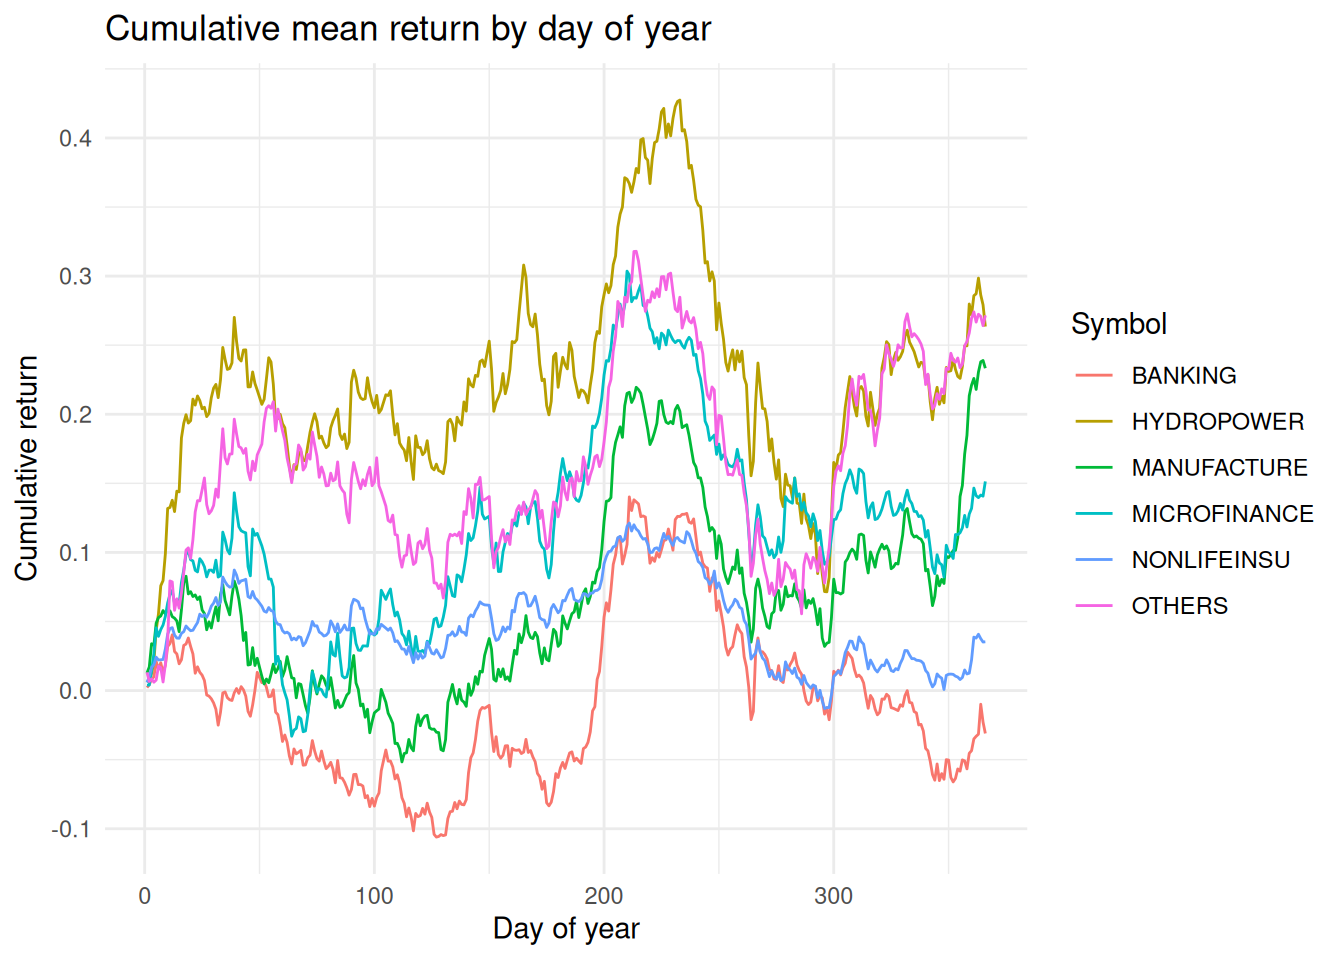
\includegraphics[width=0.95\textwidth]{figures/stats-cumalative-return-by-year.png}
\caption{Cumulative mean return by day of the year for each sector. The peak indicates the optimal exit day.}
\label{fig:cumulative}
\end{figure}

Table~\ref{tab:optimalexit} lists the optimal exit day for each sector. For Banking, Microfinance, and Non-Life Insurance, the peak occurs around day 210 (late July), aligning with the strong performance of July observed in the monthly rankings. Hydropower reaches its maximum somewhat later, at day 230 (mid-August), consistent with its extended positive period. The Others sector peaks at day 213. Manufacturing stands out with an optimal exit at day 365, implying that its cumulative returns increase almost monotonically until year-end. This pattern may reflect fiscal-year-end portfolio adjustments or data-specific effects, and warrants cautious interpretation.

\begin{table}[ht]
\centering
\caption{Optimal exit day (day of year) and corresponding cumulative mean return}
\label{tab:optimalexit}
\begin{tabular}{lcc}
\toprule
Sector & Exit Day (Approx. Date) & Cumulative Mean Return \\
\midrule
BANKING       & 210 (29 July)   & 0.113 \\
HYDROPOWER    & 230 (18 August) & 0.422 \\
MANUFACTURE   & 365 (31 December) & 0.202 \\
MICROFINANCE  & 210 (29 July)   & 0.329 \\
NONLIFEINSU   & 210 (29 July)   & 0.120 \\
OTHERS        & 213 (1 August)  & 0.265 \\
\bottomrule
\end{tabular}
\end{table}

\subsection{Year-on-Year Consistency}

Table~\ref{tab:consistency} reports the months that passed the 80\% consistency threshold. July is the most robust month, with 100\% consistency for Banking and 80\% for four other sectors. January and November also appear with high consistency for several sectors. This year-on-year reliability strengthens the case for a genuine seasonal anomaly rather than an artifact of a particular year. The fact that no month for Manufacturing reaches the 80\% threshold other than January, May, and July suggests that its seasonality is less stable than in other sectors.

\begin{table}[ht]
\centering
\caption{Months with year-on-year consistency \(\ge 0.80\)}
\label{tab:consistency}
\begin{tabular}{lccc}
\toprule
Sector & Month & Positive/Total Years & Consistency \\
\midrule
BANKING       & July    & 5/5  & 1.00 \\
\addlinespace
HYDROPOWER    & January & 6/6  & 1.00 \\
HYDROPOWER    & July    & 4/5  & 0.80 \\
HYDROPOWER    & November& 5/5  & 1.00 \\
\addlinespace
MANUFACTURE   & January & 5/6  & 0.833 \\
MANUFACTURE   & May     & 4/5  & 0.80 \\
MANUFACTURE   & July    & 4/5  & 0.80 \\
\addlinespace
MICROFINANCE  & May     & 4/5  & 0.80 \\
MICROFINANCE  & July    & 4/5  & 0.80 \\
\addlinespace
NONLIFEINSU   & May     & 4/5  & 0.80 \\
NONLIFEINSU   & July    & 4/5  & 0.80 \\
NONLIFEINSU   & November& 4/5  & 0.80 \\
\addlinespace
OTHERS        & January & 5/6  & 0.833 \\
OTHERS        & July    & 4/5  & 0.80 \\
OTHERS        & November& 5/5  & 1.00 \\
\bottomrule
\end{tabular}
\end{table}

\subsection{Bootstrap Confidence Intervals}

Table~\ref{tab:bootstrap} presents the 95\% bootstrap percentile confidence intervals for the mean return in January for each sector. The intervals for Hydropower (\(0.00263, 0.01020\)) and Others (\(0.00032, 0.00730\)) lie entirely above zero, confirming a statistically significant positive mean return in January. For Microfinance and Non-Life Insurance, the lower bounds are very close to zero, while Banking's interval straddles zero. These findings are consistent with the monthly ranking (January as a strong month for many sectors) and provide inferential support for the point estimates.

\begin{table}[ht]
\centering
\caption{Bootstrap 95\% confidence intervals for mean return in January}
\label{tab:bootstrap}
\begin{tabular}{lcc}
\toprule
Sector & Lower CI & Upper CI \\
\midrule
NONLIFEINSU  & 0.00005 & 0.00334 \\
MANUFACTURE  & -0.00170 & 0.00456 \\
BANKING      & -0.00238 & 0.00178 \\
OTHERS       & 0.00032 & 0.00730 \\
MICROFINANCE & -0.00012 & 0.00584 \\
HYDROPOWER   & 0.00263 & 0.01020 \\
\bottomrule
\end{tabular}
\end{table}

The 95\% bootstrap CI for Banking in August is \((-0.0048, 0.0004)\), which includes zero, underscoring that the negative point estimate for August is not statistically distinguishable from zero at the 5\% level. Nonetheless, the overwhelmingly negative direction across all sectors lends practical significance to avoiding long positions during this period.

\subsection{Robust ANOVA and Permutation Test}

The one-way ANOVA on 20\% trimmed means (robust ANOVA) yielded a test statistic of \(F_t = 12.2519\) with \(p < 0.001\). The effect size \(\hat{\eta} = 0.16\) (95\% bootstrap CI \([0.13, 0.19]\)) indicates a moderate-to-large effect of month on trimmed mean returns. This robust test is insensitive to outliers and heterogeneity of variance, and its significance confirms that the month effect is not an artifact of a few extreme observations.

The permutation test with 5000 random shuffles of month labels produced \(p < 2.2 \times 10^{-16}\). Because the permutation test does not rely on any distributional assumptions, it provides the strongest possible evidence that the observed monthly differences are not due to chance. Together, the robust ANOVA and permutation test reinforce the parametric and non-parametric results, establishing monthly seasonality as a genuine feature of the data.

\subsection{Two-Way Interaction ANOVA}

The two-way ANOVA crossing sector and month decomposes the variation in daily returns:
\begin{itemize}
    \item \textbf{Sector}: \(F(5, \text{large}) = 0.502\), \(p = 0.775\) — not significant.
    \item \textbf{Month}: \(F(11, \text{large}) = 10.440\), \(p < 2\times10^{-16}\) — highly significant.
    \item \textbf{Sector \(\times\) Month interaction}: \(F(55, \text{large}) = 0.702\), \(p = 0.954\) — not significant.
\end{itemize}
The absence of a significant interaction implies that the monthly pattern of returns is essentially the same across the six sectors. In other words, the seasonal highs and lows occur in the same calendar months for all sectors, although the magnitude of the effect may differ slightly. This justifies the use of a unified seasonal trading calendar with only minor sector-specific adjustments (e.g., the later exit for Hydropower).

\subsection{Summary of Key Findings and Practical Implications}

The empirical results provide robust, multi-method evidence of pronounced monthly seasonality in NEPSE sub-sector returns, consistent with the findings of \cite{gurung2024fiscal}, \cite{rijal2025turn}, and \cite{shrestha2023seasonal}. Several key insights emerge that are of practical importance to investors:

\begin{itemize}
    \item \textbf{July (Shrawan) as the premier seasonal window.} July records the highest mean returns across five of six sectors, with win ratios exceeding 60\% and perfect year-on-year consistency for Banking. The new fiscal year budget announcements and institutional portfolio rebalancing at the start of the fiscal year are plausible drivers of this effect. Both the Z-score framework (ENTRY signals in preceding months) and the cumulative return analysis (peak around day 210) identify late July as an optimal exit point.
    
    \item \textbf{August–September decline.} August and September consistently show negative mean returns, low win ratios, and negative Sharpe ratios. This pattern aligns with profit booking ahead of the Dashain festival and pre-festival liquidity constraints. The absence of a significant sector–month interaction indicates that the August–September weakness affects all sectors uniformly, making a broad market-timing strategy feasible.
    
    \item \textbf{Optimal exit timing.} The cumulative return curves peak between day 210 and 213 for most sectors, suggesting that investors should close positions in late July or very early August. Hydropower's later peak (day 230, mid-August) may reflect its different investor base or sector-specific news flow. The Manufacturing sector's year-end peak could reflect a data artifact (e.g., thin trading at year-end) or a genuine end-of-calendar-year effect; caution is advised when extrapolating this pattern.
    
    \item \textbf{Z-score trading signals.} The average ENTRY Z-score of approximately -2.0, combined with the high excess kurtosis in all sectors, suggests that a more conservative threshold of \(\pm 1.8\) would reduce false signals while still capturing meaningful oversold conditions. The framework can be operationalised by monitoring daily Z-scores and taking positions when the threshold is breached, with risk management rules to account for the fat-tailed nature of returns.
    
    \item \textbf{Consistency and robustness.} The year-on-year consistency analysis isolates months that are not only historically profitable on average but also reliably so. July, January, and November appear as the most consistent months across sectors. The robustness checks (robust ANOVA, permutation test, bootstrap CIs) confirm that these findings are not driven by outliers or distributional assumptions.
    
    \item \textbf{Sectoral uniformity.} The non-significant interaction in the two-way ANOVA suggests that, contrary to the expectation of sector-specific fiscal-year-end effects, the seasonal pattern is largely common across sectors. This implies that a single seasonal calendar can be applied to the broad NEPSE index or to a diversified portfolio, with minimal sector-specific tilts (e.g., a slightly extended holding period for Hydropower).
\end{itemize}

\noindent
\textbf{Overall key finding:} July (Shrawan) stands out as the best month across virtually all NEPSE sub-sectors, with high mean returns, favourable risk-adjusted metrics, and perfect or near-perfect year-on-year consistency. August and September are the worst months, and the optimal exit window is late July to mid-August. These patterns challenge the weak-form efficiency of the Nepalese stock market and provide a practical, evidence-based seasonal trading calendar.

\section{Conclusion}

This study applied a comprehensive battery of statistical and econometric methods—ranging from exploratory visualisation and distributional analysis to parametric, non-parametric, robust, and resampling tests—to investigate seasonal patterns in six NEPSE sub-sectors from 2021 to 2026. The principal conclusions are:

\begin{enumerate}
    \item \textbf{Strong monthly seasonality.} The chi-square test of independence, one-way ANOVA, Kruskal–Wallis test, robust ANOVA on trimmed means, and permutation test all converge on the finding of highly significant monthly variation in returns (\(p < 0.001\)). This seasonality is not an artifact of outliers or distributional assumptions.
    
    \item \textbf{July as the optimal entry month.} July (Shrawan) delivers the highest mean returns (up to 0.599\% per day), win ratios above 60\%, and 100\% consistency for the Banking sector. It is the single best month for five of the six sectors and a strong second for Hydropower.
    
    \item \textbf{August–September as the avoidance window.} These two months exhibit uniformly negative returns, low win rates, and negative Sharpe ratios across all sectors, making them unattractive for long-only strategies.
    
    \item \textbf{Optimal exit timing.} The cumulative return analysis identifies day 210–213 (late July–early August) as the historical exit point for most sectors. Hydropower benefits from a slightly later exit (day 230, mid-August), while Manufacturing shows a year-end peak that requires further investigation.
    
    \item \textbf{Z-score framework generates actionable signals.} Standardising returns within sector–months and applying a \(Z < -1.5\) entry threshold identifies oversold conditions, with an average signal strength near -2.0. Given the fat tails, a more conservative threshold of \(\pm 1.8\) is recommended.
    
    \item \textbf{Sector-invariant seasonal pattern.} The non-significant sector–month interaction in the two-way ANOVA indicates that the seasonal calendar is largely uniform across sectors. A single seasonal strategy, with minor adjustments for Hydropower and Manufacturing, can be applied broadly.
\end{enumerate}

These findings challenge the weak-form efficiency of the Nepal Stock Exchange, as they imply that historical price patterns contain exploitable information about future returns \cite{basnet2022efficient, adhikari2024calendar, sharma2021investor}. While the presence of seasonality does not guarantee future profits—transaction costs, market impact, and structural changes could erode returns—the robustness of the evidence across multiple methods and sectors strengthens the case for incorporating seasonal timing into investment decisions. Future research could extend this analysis to intra-sector dynamics, test out-of-sample predictability, and explore the macroeconomic and institutional drivers behind the observed calendar anomalies.

\appendix
\section*{Appendix A: Complete R Code Used in this Project}

\subsection*{Data Loading and Exploratory Analysis}
\begin{tcolorbox}[colback=gray!5, colframe=black!70, fontupper=\small, breakable, title=R Code]
\begin{verbatim}
library(dplyr)
library(ggplot2)
nepse_data <- read.csv("./data/nepse.csv")
nepse_data <- nepse_data |> mutate(Date = as.Date(Date)) |> arrange(Date)
head(nepse_data, 5)

ggplot(nepse_data, aes(x = Symbol, y = Close, fill = Symbol)) +
  geom_boxplot() +
  labs(title = "Box Plot of Close Price by Symbol", 
       x = "Symbol", y = "Close Price") +
  theme_minimal() + 
  theme(axis.text.x = element_text(angle = 45, hjust = 1))

ggplot(nepse_data, aes(x = Close, fill = Symbol)) +
  geom_histogram(bins = 30, color = "white") +
  facet_wrap(~Symbol, scales = "free") +
  labs(title = "Histogram of Close Price by Symbol",
       x = "Close Price", y = "Frequency") +
  theme_minimal()

ggplot(nepse_data, aes(sample = Close, color = Symbol)) +
  stat_qq() + stat_qq_line() +
  facet_wrap(~Symbol, scales = "free") +
  labs(title = "Q-Q Plot of Close Price by Symbol",
       x = "Theoretical Quantiles", y = "Sample Quantiles") +
  theme_minimal()
\end{verbatim}
\end{tcolorbox}

\subsection*{Return Calculation and Distribution}
\begin{tcolorbox}[colback=gray!5, colframe=black!70, fontupper=\small, breakable, title=R Code]
\begin{verbatim}
library(moments)
library(lubridate)

sector_returns <- nepse_data |>
  group_by(Symbol) |> arrange(Date) |>
  mutate(Return = (Close - lag(Close)) / lag(Close)) |>
  filter(!is.na(Return))

distribution_stats <- sector_returns |>
  summarise(Mean = mean(Return), SD = sd(Return),
            Skewness = skewness(Return), Kurtosis = kurtosis(Return))
print(distribution_stats)

normality_sw <- sector_returns |>
  group_by(Symbol) |>
  summarise(p_value = shapiro.test(Return)$p.value)
print(normality_sw)
\end{verbatim}
\end{tcolorbox}

\subsection*{Additional Exploratory Visualizations}
\begin{tcolorbox}[colback=gray!5, colframe=black!70, fontupper=\small, breakable, title=R Code]
\begin{verbatim}
# 1. Monthly bar plot with bootstrap CIs
monthly_stats <- sector_returns |>
  mutate(Month = month(Date, label = TRUE)) |>
  group_by(Symbol, Month) |>
  summarise(Mean = mean(Return),
            CI_lower = quantile(Return, 0.025),
            CI_upper = quantile(Return, 0.975),
            .groups = "drop")

ggplot(monthly_stats, aes(x = Month, y = Mean, fill = Symbol)) +
  geom_col(position = position_dodge(0.9), color = "black", alpha = 0.7) +
  geom_errorbar(aes(ymin = CI_lower, ymax = CI_upper),
                position = position_dodge(0.9), width = 0.3) +
  geom_hline(yintercept = 0, linetype = "dashed", color = "red") +
  facet_wrap(~Symbol, scales = "free_y") +
  labs(title = "Monthly Average Daily Returns with 95% Bootstrap CIs",
       x = "Month", y = "Mean Return") +
  theme_minimal() +
  theme(axis.text.x = element_text(angle = 45, hjust = 1),
        legend.position = "none")
# Save: ggsave("figures/stats-monthly-bar.png", width = 10, height = 6)

# 2. Density plots with normal reference
norm_params <- sector_returns |>
  group_by(Symbol) |>
  summarise(mu = mean(Return), sigma = sd(Return))

ggplot(sector_returns, aes(x = Return, fill = Symbol)) +
  geom_density(alpha = 0.4, adjust = 1.5) +
  geom_function(fun = dnorm, 
                args = list(mean = first(norm_params$mu), 
                            sd = first(norm_params$sigma)),
                color = "red", linetype = "dotted", size = 1) +
  facet_wrap(~Symbol, scales = "free") +
  labs(title = "Return Density Plots with Normal Reference (dotted red)",
       x = "Daily Return", y = "Density") +
  theme_minimal() +
  theme(legend.position = "none")
# Save: ggsave("figures/stats-density.png", width = 10, height = 6)

# 3. Cumulative time series
cumulative_returns <- sector_returns |>
  group_by(Symbol) |>
  arrange(Date) |>
  mutate(Cumulative = cumsum(Return)) |>
  ungroup()

ggplot(cumulative_returns, aes(x = Date, y = Cumulative, color = Symbol)) +
  geom_line(size = 0.8) +
  labs(title = "Cumulative Daily Returns by Sector (2021–2026)",
       x = "Date", y = "Cumulative Return") +
  theme_minimal() +
  theme(legend.position = "bottom")
# Save: ggsave("figures/stats-cumulative-ts.png", width = 10, height = 5)

# 4. Heatmap
heatmap_data <- sector_returns |>
  mutate(Month = month(Date, label = TRUE)) |>
  group_by(Symbol, Month) |>
  summarise(Mean_Return = mean(Return), .groups = "drop")

ggplot(heatmap_data, aes(x = Month, y = Symbol, fill = Mean_Return)) +
  geom_tile(color = "white") +
  scale_fill_gradient2(low = "red", mid = "white", high = "steelblue",
                       midpoint = 0, name = "Mean Return") +
  geom_text(aes(label = round(Mean_Return, 4)), color = "black", size = 3) +
  labs(title = "Heatmap of Average Daily Returns by Sector and Month",
       x = "Month", y = "Sector") +
  theme_minimal() +
  theme(axis.text.x = element_text(angle = 45, hjust = 1))
# Save: ggsave("figures/stats-heatmap.png", width = 8, height = 5)

# 5. ACF plots (using forecast package)
library(forecast)
library(purrr)
acf_data <- sector_returns |>
  group_by(Symbol) |>
  summarise(acf_list = list(acf(Return, plot = FALSE, lag.max = 20))) |>
  mutate(acf_df = map(acf_list, ~ data.frame(Lag = .x$lag, ACF = .x$acf))) |>
  unnest(acf_df)

ggplot(acf_data, aes(x = Lag, y = ACF)) +
  geom_bar(stat = "identity", fill = "steelblue", alpha = 0.7) +
  geom_hline(yintercept = 0) +
  geom_hline(yintercept = c(-0.05, 0.05), linetype = "dashed", color = "red") +
  facet_wrap(~Symbol) +
  labs(title = "Autocorrelation Function (ACF) by Sector",
       x = "Lag", y = "Autocorrelation") +
  theme_minimal()
# Save: ggsave("figures/stats-acf.png", width = 10, height = 6)
\end{verbatim}
\end{tcolorbox}

\subsection*{Regression Models}
\begin{tcolorbox}[colback=gray!5, colframe=black!70, fontupper=\small, breakable, title=R Code]
\begin{verbatim}
linear_model <- lm(Return ~ as.numeric(Date), data = sector_returns)
summary(linear_model)

model_data <- sector_returns |>
  group_by(Symbol) |> mutate(Lag_Return = lag(Return)) |>
  filter(!is.na(Lag_Return))
multi_reg <- lm(Return ~ Lag_Return + Symbol, data = model_data)
summary(multi_reg)
\end{verbatim}
\end{tcolorbox}

\subsection*{Chi-Square and ANOVA}
\begin{tcolorbox}[colback=gray!5, colframe=black!70, fontupper=\small, breakable, title=R Code]
\begin{verbatim}
chi_data <- sector_returns |>
  mutate(Direction = ifelse(Return > 0, "Gain", "Loss"),
         Month = month(Date, label = TRUE))
ctable <- table(chi_data$Month, chi_data$Direction)
chisq_test <- chisq.test(ctable); print(chisq_test)

anova_month <- aov(Return ~ factor(month(Date)), data = sector_returns)
summary(anova_month)
anova_sector <- aov(Return ~ Symbol, data = sector_returns)
summary(anova_sector)
\end{verbatim}
\end{tcolorbox}

\subsection*{Non-Parametric Tests}
\begin{tcolorbox}[colback=gray!5, colframe=black!70, fontupper=\small, breakable, title=R Code]
\begin{verbatim}
kw_test <- kruskal.test(Return ~ Symbol, data = sector_returns); print(kw_test)
subset_data <- sector_returns |> filter(Symbol %in% c("BANKING", "OTHERS"))
mw_test <- wilcox.test(Return ~ Symbol, data = subset_data); print(mw_test)
\end{verbatim}
\end{tcolorbox}

\subsection*{Seasonality Analysis}
\begin{tcolorbox}[colback=gray!5, colframe=black!70, fontupper=\small, breakable, title=R Code]
\begin{verbatim}
library(boot)
library(WRS2)
library(lmPerm)
library(tidyr)
library(purrr)

monthly_returns <- sector_returns |>
  mutate(Month = month(Date, label = TRUE)) |>
  group_by(Symbol, Month) |>
  summarise(Mean_Return = mean(Return), Median_Return = median(Return),
            CI_Lower = quantile(Return, 0.025), CI_Upper = quantile(Return, 0.975),
            Win_Ratio = sum(Return > 0)/n(), Sharpe = mean(Return)/sd(Return),
            .groups = "drop")
best_months <- monthly_returns |> group_by(Symbol) |> slice_max(Mean_Return, n=2)
worst_months <- monthly_returns |> group_by(Symbol) |> slice_min(Mean_Return, n=2)

zscore_analysis <- sector_returns |>
  mutate(Month = month(Date, label = TRUE)) |>
  group_by(Symbol, Month) |>
  mutate(Monthly_Mean = mean(Return), Monthly_SD = sd(Return),
         Z_Score = (Return - Monthly_Mean)/Monthly_SD) |> ungroup()
signals <- zscore_analysis |> filter(abs(Z_Score) > 1.5) |>
  mutate(Signal = ifelse(Z_Score < -1.5, "ENTRY", "EXIT")) |>
  group_by(Symbol, Signal, Month) |>
  summarise(Frequency = n(), Avg_Z = mean(Z_Score))

cumulative_pattern <- sector_returns |>
  mutate(DayOfYear = yday(Date)) |>
  group_by(Symbol, DayOfYear) |> 
  summarise(Mean_Return = mean(Return), .groups="drop") |>
  group_by(Symbol) |> mutate(Cumulative_Mean = cumsum(Mean_Return))
optimal_exit <- cumulative_pattern |> group_by(Symbol) |>
  slice_max(Cumulative_Mean, n=1) |> mutate(Exit_Day = DayOfYear)

consistency_test <- sector_returns |>
  mutate(Year = year(Date), Month = month(Date, label=TRUE)) |>
  group_by(Symbol, Month, Year) |>
  summarise(Monthly_Return = sum(Return), .groups="drop") |>
  group_by(Symbol, Month) |>
  summarise(Positive_Years = sum(Monthly_Return > 0), Total_Years = n(),
            Consistency_Rate = Positive_Years/Total_Years, .groups="drop") |>
  filter(Total_Years >= 3)
reliable_seasons <- consistency_test |> filter(Consistency_Rate >= 0.8)

boot_mean <- function(x, indices) mean(x[indices], na.rm=TRUE)
sector_months <- sector_returns |>
  distinct(Symbol, Month = month(Date)) |>
  mutate(Returns_list = map2(Symbol, Month, ~ 
            filter(sector_returns, Symbol==.x, month(Date)==.y) |>
            pull(Return)))
bootstrap_results <- sector_months |>
  mutate(Boot = map(Returns_list, ~ {
    if(length(.x)<2) return(tibble(CI_lower=NA, CI_upper=NA))
    set.seed(123); b <- boot(.x, boot_mean, R=1000)
    ci <- tryCatch(boot.ci(b, type="perc")$percent[4:5], 
                   error=function(e) c(NA,NA))
    tibble(CI_lower=ci[1], CI_upper=ci[2])
  })) |> unnest(Boot)

robust_anova_month <- t1way(Return ~ factor(month(Date)),
                            data=sector_returns, tr=0.2)
set.seed(123)
perm_anova_month <- aovp(Return ~ factor(month(Date)), 
                         data=sector_returns, np=1000)

sector_returns <- sector_returns |> mutate(MonthFactor = factor(month(Date)))
interaction_anova <- aov(Return ~ Symbol * MonthFactor, data=sector_returns)
summary(interaction_anova)
\end{verbatim}
\end{tcolorbox}

\bibliographystyle{unsrt}
\bibliography{references}

\end{document}